\documentclass[polish,12pt,titlepage]{article}

\usepackage{graphicx}
\usepackage{graphics}
\usepackage{amsmath}
\usepackage{amssymb}
\usepackage{amsthm}
\usepackage{booktabs}
\usepackage{stmaryrd}
\usepackage{url}
\usepackage{hyperref}
\usepackage{longtable}
\usepackage[figuresright]{rotating}

\usepackage[utf8]{inputenc}
\usepackage[T1]{fontenc}
\usepackage[polish]{babel}
\selectlanguage{polish}

\usepackage{pslatex}
\usepackage{ulem}
\usepackage[htt]{hyphenat}

\usepackage{listings}
\usepackage{url}
\usepackage{path}
\usepackage{here}

\usepackage{color}
\definecolor{lightgray}{gray}{0.6}

%\setlength{\textwidth}{400pt}

\lstset{numbers=left,
			numberstyle=\tiny, 
			basicstyle=\scriptsize\ttfamily, 
			breaklines=true, 
			captionpos=b, 
			tabsize=2}

\usepackage[ruled,vlined,linesnumbered]{algorithm2e}

\newcommand{\RR}{\mathbb{R}}
\newcommand{\NN}{\mathbb{N}}
\newcommand{\QQ}{\mathbb{Q}}
\newcommand{\ZZ}{\mathbb{Z}}
\newcommand{\TAB}{\hspace{0.50cm}}
\newcommand{\IFF}{\leftrightarrow}
\newcommand{\IMP}{\rightarrow}

\newtheorem{theorem}{Theorem}[section]
\newtheorem{lemma}{Lemma}[section]
\newtheorem{example}{Example}[section]
\newtheorem{corollary}{Corollary}[section]
\newtheorem{definition}{Definition}[section]

\makeindex

\begin{document}

\pagestyle{empty}

%%%%%%%%%%%%%%%%%%%%%%%%%%%%%%%%%%%%%%%%%%%%%%%%%%%%%%%%%%%%%%%%%%%%%%%%%%%%%%
%%%%%%%%%%%%%%%%%%%%%%%%%%%%%%%% TITLE PAGE %%%%%%%%%%%%%%%%%%%%%%%%%%%%%%%%%%
%%%%%%%%%%%%%%%%%%%%%%%%%%%%%%%%%%%%%%%%%%%%%%%%%%%%%%%%%%%%%%%%%%%%%%%%%%%%%%

\begin{titlepage}
\vspace*{\fill}
\begin{center}
\begin{picture}(500,500)
  \put( 10,520){\makebox(0,0)[l]{\large \bf \textsc{Wydział Podstawowych Problemów Techniki}}}
  \put( 10,500){\makebox(0,0)[l]{\large \bf \textsc{Politechniki Wrocławskiej}}}
  
  \put(180,280){\makebox(0,0)[l]{\Huge  \bf \textsc{Klient serwera}}}
  \put(180,260){\makebox(0,0)[l]{\Huge  \bf \textsc{do aktualizacji}}} 
  \put(180,240){\makebox(0,0)[l]{\Huge  \bf \textsc{oprogramowania}}}
  \put(200,200){\makebox(0,0)[l]{\large     \textsc{Mateusz Jakub Kubuszok}}}

  \put(180, 80){\makebox(0,0)[l]{\large  {Praca inżynierska napisana}}}
  \put(180, 60){\makebox(0,0)[l]{\large  {pod kierunkiem}}}
  \put(180, 40){\makebox(0,0)[l]{\large  {dr. inż. Marcina Zawady}}}

  \put(100,-40){\makebox(0,0)[bl]{\large \bf \textsc{Wrocław 2013}}}
\end{picture}
\end{center}
\vspace*{\fill}
\end{titlepage}

%%%%%%%%%%%%%%%%%%%%%%%%%%%%%%%%%%%%%%%%%%%%%%%%%%%%%%%%%%%%%%%%%%%%%%%%%%%%%%
%%%%%%%%%%%%%%%%%%%%%%%%%%%% TABLE OF CONTENTS %%%%%%%%%%%%%%%%%%%%%%%%%%%%%%%
%%%%%%%%%%%%%%%%%%%%%%%%%%%%%%%%%%%%%%%%%%%%%%%%%%%%%%%%%%%%%%%%%%%%%%%%%%%%%%

\tableofcontents

\newpage

\pagestyle{headings}

%%%%%%%%%%%%%%%%%%%%%%%%%%%%%%%%%%%%%%%%%%%%%%%%%%%%%%%%%%%%%%%%%%%%%%%%%%%%%%
%%%%%%%%%%%%%%%%%%%%%%%%%%%%%%% INTRODUCTION %%%%%%%%%%%%%%%%%%%%%%%%%%%%%%%%%
%%%%%%%%%%%%%%%%%%%%%%%%%%%%%%%%%%%%%%%%%%%%%%%%%%%%%%%%%%%%%%%%%%%%%%%%%%%%%%

\section*{Wstęp}

Celem projektu jest stworzenie aplikacji, która będzie dokonywać aktualizacji
określonych programów, na podstawie lokalnych danych oraz informacji pobranych 
z repozytorium (udostępnionego do projektu jako implementacja wzorcowa). 
Efekt końcowy będzie wykorzystywany w oddziałach Nokia Siemens Networks, tak 
przez programistów wewnętrznych narzędzi jak i ich użytkowników.

W rozdziale ,,Specyfikacje funkcjonalna i niefunkcjonalna'' zdefiniowano
wymagania postawione przed projektem, zdefiniowane przez przedsiębiorstwo
Nokia Siemens Networks.

W rozdziale ,,Analiza problemu'' przeprowadzono analizę założeń, aby wiedzieć
jakie środki będą potrzebne do doprowadzenia projektu do końca już na etapie
planowania.

W rozdziale ,,Projekt klienta AutoUpdatera'' omówiono założenia projektu,
przedstawiono szkicowe diagramy UML przyszłych klas oraz diagramy sekwencji
ilustrujące planowany przebieg instalacji.

W rozdziale ,,Implementacja'' omówiono najważniejsze informacje na temat
działania projektu, w tym kluczowe szczegóły implementacji.

Rozdział ,,Instalacja i wdrożenie'' opisuje sposób wykorzystania gotowej
biblioteki.

\newpage

%%%%%%%%%%%%%%%%%%%%%%%%%%%%%%%%%%%%%%%%%%%%%%%%%%%%%%%%%%%%%%%%%%%%%%%%%%%%%%
%%%%%%%%%%%%%%%%%%%%%%%%%%%%%%% SPECIFICATION %%%%%%%%%%%%%%%%%%%%%%%%%%%%%%%%
%%%%%%%%%%%%%%%%%%%%%%%%%%%%%%%%%%%%%%%%%%%%%%%%%%%%%%%%%%%%%%%%%%%%%%%%%%%%%%

\section{Specyfikacje: funkcjonalna i niefunkcjonalna}

Zdefiniowano następujące wymagania funkcjonalne:
\begin{enumerate}
  \item automatyczne kończenie uruchomionych instancji aktualizowanych
    programów,
  \item rozróżnienie na wersji produkcyjnej oraz rozwojowej - każda ma
    istnieć jako osobna wersja, z osobnymi aktualizacjami, instalowanymi tylko
    dla wybranej wersji,
  \item podział programów na pakiety, gdzie każdy pakiet będzie wersjonowany
    osobno,
  \item klient powinien być obsługiwany z poziomu graficznego interfejsu
    użytkownika (GUI),
  \item kod klienta powinien być rozwijany jako samodzielna biblioteka,
    GUI ma jedynie wykorzystywać jej funkcjonalność,
  \item dla każdej aktualizacji powinna zdefiniowana jedna z 3 strategii jej
    przeprowadzenia:
  \begin{itemize}
    \item kopia - kopia pobranego pliku jest tworzona w wybranej lokalizacji
      katalogu instalacji,
    \item ekstrakcja - wypakowuje zawartość pobranego pliku do wybranej
      lokalizacji katalogi instalacji,
    \item wykonanie - wywołuje pobraną aktualizację jako plik wykonywalny,
  \end{itemize}
  \item klient powinien być w stanie wyświetlić listę znanych błędów dla
    danego programu, oraz listy zmian dla danego pakietu.
\end{enumerate}

Specyfikacja niefunkcjonalna jest zdefiniowana w następujący sposób:
\begin{enumerate}
  \item wymagane jest wsparcie zarówno rodziny systemów Windows jak i Linux,
  \item ze względu na możliwość przyszłych żądań zmian (w GUI) kod biblioteki
    powinien być możliwe elastyczny,
  \item wymagane jest stosowanie testów jednostkowych,
  \item wymagana jest pełna dokumentacja projektu (Javadoc),
  \item wymaganą platformą jest Java SE (najlepiej w wersji 1.7).
\end{enumerate}

Ponieważ nie istnieją zewnętrzne programy, które można łatwo dostosować do
formatu repozytoriów dostarczonego przez Nokia Siemiens Networks, konieczne
jest stworzenie klienta, który będzie potrafił je wykorzystać.

\newpage

%%%%%%%%%%%%%%%%%%%%%%%%%%%%%%%%%%%%%%%%%%%%%%%%%%%%%%%%%%%%%%%%%%%%%%%%%%%%%%
%%%%%%%%%%%%%%%%%%%%%%%%%%%%%%%%% ANALYSIS %%%%%%%%%%%%%%%%%%%%%%%%%%%%%%%%%%%
%%%%%%%%%%%%%%%%%%%%%%%%%%%%%%%%%%%%%%%%%%%%%%%%%%%%%%%%%%%%%%%%%%%%%%%%%%%%%%

\section{Analiza problemu}

Biblioteka powinna być w stanie wykonywać dwa rodzaje zadań zależnych od
użytego systemu: utworzenie procesu (z uprawnieniami administratora) oraz
zabicie procesu. Pierwsze jest konieczne do przeprowadzenia właściwego procesu
aktualizacji - kopiowania i nadpisywania plików, oraz wykonywania programów.
Drugie jest wymagane do zakończenia pracy aktualizowanych programów.

Ponieważ Java jest niezależna od platformy systemowej (i sprzętowej) nie
zaimplementowano w niej usług specyficznych dla danego systemu
operacyjnego, tj. nabywania uprawnień \cite{JAVA_VISTA_UPRAWNIENIA} i
zabijania procesów nie utworzonych przez samą maszynę wirtualną. Z tego
powodu oba te zadania będą musiały zostać zaimplementowane dla każdego
systemu osobno, z wykorzystaniem narzędzi udostępnionych na danej platformie.
O tym, która implementacja powinna zostać używa, biblioteka powinna
zadecydować w czasie uruchomienia.

Zarówno dane lokalne jak i te pochodzące z repozytorium, mogą zostać
przestawione jako pewne obiekty, ich kolekcje zaś agregowane przy pomocy
zbiorów uporządkowanych (\texttt{SortedSet}) - zapewniałyby one unikalność
danej instancji w kolekcji, a także umożliwiały szybkie porównywanie obiektów.
Z tego powodu każdy model musiałby mieć zdefiniowaną relację równoważności
oraz porządku liniowego (przeciążenie metod \texttt{equal(Object)},
\texttt{hashcode()}, oraz \texttt{compareTo(Object)}).

Ze względu na możliwość potencjalnych przyszłych zmian w GUI, biblioteka 
powinna być możliwie elastyczna, pozwalając programiście dowolnie wybierać, 
które aktualizacje powinny zostać pobrane i zainstalowane. Powinna również
mieć zaimplementowaną obsługę błędów na wszystkich etapach zarządzania
lokalną instalacją, wykonywania zapytań do repozytoriów jak również
pobierania i instalacji aktualizacji.

Testy jednostkowe dla zwiększenia przejrzystości powinny wykorzystywać
którąś z zewnętrznych bibliotek wspomagających pisanie asercji, ponieważ
udostępniają one metody do definiowania wielu powszechnie stosowanych asercji
o czytelnych nazwach, umożliwiających szybkie rozumienie czytanego kodu.
Testy powinny również wykorzystywać jakąś bibliotekę do tworzenia obiektów
mockowych - specjalnych instancji, używanych tylko w testach - tam, gdzie 
potrzeba jest implementacja złożonego interfejsu lub gwarancja braku efektów 
ubocznych na stan środowiska poza klasą testującą.

Istniejące biblioteki zewnętrzne, które zdobyły już uznanie programistów,
powinny zostać zastosowane do przyspieszenia rozwoju projektu i uniknięcia
tworzenia zbędnego kodu poprzez wykorzystanie dobrze zaprojektowanych,
przetestowanych i udokumentowanych klas do wykonywania często spotykanych
zadań, takich jak parsowanie dokumentów XML, zarządzanie plikami i oraz
operacje na kolekcjach. W szczególności mogą być one wykorzystane do
parsowania danych pobranych z serwera, jako że są one zwracane w formacie
XML.

Biblioteka powinna lokalnie przechowywać dane takie jak: które programy
i pakiety są zainstalowane, jakie są ich wersje i jakie są adresy ich
repozytoriów. Z serwerów powinna pobierać dane na temat programów oraz
pakietów dostępnych do pobrania i ograniczać je do programów przeznaczonych
do instalacji/aktualizacji. Powinna istnieć możliwość wyboru, które
z pakietów mają być sprawdzone pod kątem możliwości instalacji/aktualizacji.
Następnie, możliwość dokonania wyboru aktualizacji do instalacji, spośród
wszystkich pobranych. Taka nadmiarowa zdolność do kontroli działania
biblioteki dawałaby programiście możliwość dokładnego określenia przebiegu
całego procesu aktualizacji. On też zdecydowałby jak duży wpływ na wybór w
poszczególnych etapach miałby użytkownik końcowy.

Na każdym kroku każdego z tych procesów, programista powinien być w stanie
uzyskać informację na temat stanu bieżącej operacji.

\newpage

%%%%%%%%%%%%%%%%%%%%%%%%%%%%%%%%%%%%%%%%%%%%%%%%%%%%%%%%%%%%%%%%%%%%%%%%%%%%%%
%%%%%%%%%%%%%%%%%%%%%%%%%%%%%%%%%% PROJECT %%%%%%%%%%%%%%%%%%%%%%%%%%%%%%%%%%%
%%%%%%%%%%%%%%%%%%%%%%%%%%%%%%%%%%%%%%%%%%%%%%%%%%%%%%%%%%%%%%%%%%%%%%%%%%%%%%

\section{Projekt aplikacji do aktualizacji oprogramowania}


\subsection{Docelowi użytkownicy oraz założenia}

Możemy wyróżnić dwie grupy docelowe użytkowników: programiści oraz zwykli
użytkownicy dystrybuowanych programów. Programiści wymagają możliwości
stosowania ciągłej integracji, przekładającej się na częste wewnętrzne wydania
kolejnych wersji ich programów w wersji rozwojowej. Może ona zawierać np.
,,debug symbols'' \footnote{Dodatkowe informacji na temat fragmentu kodu, z
którego utworzono dany kod wynikowy, generowane przez kompilator.}, jak
również inne narzędzia nie przewidziane do wykorzystania przez użytkownika
końcowego. Z kolei zwykli użytkownicy wymagają  jedynie wydań wersji
produkcyjnych, udostępnianych zazwyczaj raz na ,,sprint'' \footnote{W
rozumieniu metodologii zwinnych, zamknięty okres trwający zwykle od 1 tygodnia 
do 1 miesiąca, przewidziany na wdrożenie wybranej, z góry określonej części
funkcjonalności.}. Wyjątek stanowią łatki i poprawki bezpieczeństwa,
naprawiające krytyczne błędy, wymagające usunięcia tak szybko jak to możliwe.

W efekcie każda aktualizacja wymaga oznaczenia jako wersja produkcyjna bądź
rozwojowa. Ta zasada ma również zastosowane do danych lokalnej instalacji
programu - każdy musi być definiowany jako wersja produkcyjna bądź rozwojowa.
Dzięki temu można z góry odfiltrować aktualizacje, tak aby do danego pakietu
przypisano tylko te które są kompatybilne z zawierającym go programem.

Każdy pakiet może być traktowany jako rdzeń aplikacji, bądź dołączany do niego
moduł, lub też część dystrybucji w jakiś inny sposób niezależna od wydań jej
pozostałej części. Z tego powodu wersjonowanie odbywa się na poziomie pakietu.

Sama biblioteka powinna aktualizować nie tylko zamknięte programy, ale również
te uruchomione w czasie rozpoczęcia instalacji poprzez zakończenie ich
procesów. Dla wygody użytkowników powinna istnieć też możliwość ponownego
uruchomienia programów z użyciem biblioteki.


\subsection{Diagramy klas}

Tam, gdzie to możliwe kierunek rozwoju projektu powinien być wyznaczany
z uwzględnieniem następujących zasad:
\begin{itemize}
  \item ,,Nie powtarzaj się'' (Don't Repeat Yourself, DRY) - ograniczając
    duplikację logiki programu, redukujemy ilość miejsc gdzie może wystąpić
    błąd, oraz ilość testów jakie musimy napisać. Jednocześnie ewentualny błąd
    trzeba będzie poprawić tylko w jednym miejscu w kodzie, aby go
    wyeliminować \cite{DRY},
  \item Zasada Jednej Odpowiedzialności (Single Responsibility Principle) - 
    gwarantując, że klasa służy wyłącznie jednemu celowi unikamy ryzyka
    stworzenia Bloba, jednocześnie czyniąc kod bardziej zrozumiałym, gdyż
    klasa nie przejawia żadnych nieoczekiwanych zachowań \cite{OOD},
  \item samodokumentacja kodu \footnote{Tworzenie kodu tak, aby nazwy funkcji, 
    metod i zmiennych opisywały ich zadanie.} (w połączenie z dokumentacją 	
    Javadoc) zwiększa czytelność i ułatwia utrzymanie kodu, gdyż lepiej jest
    rozumieć kod przez samo czytanie go, bez potrzeby dodatkowego czytania
    dokumentacji każdej metody,
  \item kompozycja nad dziedziczenie - unikając głębokiego dziedziczenia
    i oddelegowując logikę do osobnej klasy, sprawiamy, że kod jest
    czytelniejszy i łatwiejszy w utrzymaniu,
  \item wykorzystanie wzorców projektowych tam, gdzie jest to uzasadnione - 
    ponieważ spora część problemów związanych z projektowaniem programu jest
    powszechnie znana i dobrze opisana, jest wysoce zalecane zastosowanie
    sprawdzonych, ogólnie przyjętych i sprawdzonych rozwiązań, zamiast tworzyć
    nowe, które najpewniej byłyby gorsze niż już istniejące. Co więcej
    stosowanie dobrze udokumentowanych wzorców projektowych, automatycznie
    dostarcza pewnych informacji na temat działania fragmentu kodu,
    w którym je wykorzystano.
\end{itemize}

Te zasady stworzone przez lata doświadczeń znakomitych programistów pozwalają
na łatwiejsze utrzymanie kodu i zmniejszenie ilości potencjalnych błędów przez
sam sposób fragmentowania kodu na klasy i metody. Poprzez przestrzeganie tych
zasad od samego początku, pośrednio zwiększamy tempo rozwoju projektu, zaś
bezpośrednio poprawiamy jego jakość.

Aby dodatkowo zwiększyć czytelność kodu, wprowadzone zostanie następująca
konwencja nazewnicza:
\begin{itemize}
  \item nazwa interfejsu powinna się zaczynać od prefiksu ,,I'', np.
    \texttt{IProcessKiller},
  \item nazwa typu wyliczeniowego powinna zaczynać się od prefiksu ,,E'', np.
    \texttt{EOperationgSystem},
  \item nazwa klasy abstrakcyjnej powinna zaczynać się od prefiksu
     ,,Abstract'', np. \texttt{AbstractDownloadService},
  \item klasy implementujące interfejs powinny zawierać część jego nazwy
    następujące po prefiksie ,,I'' jako część własnej nazwy, np.
    \texttt{WindowsProcessKiller} i \texttt{LinuxProcessKiller} są
    implementacjami interfejsu \texttt{IProcessKiller},
  \item klasy rozszerzające klasę abstrakcyjną powinny zawierać część jej
    nazwy następującą po prefiksie ,,Abstract'' jako część własnej nazwy,
    chyba, że taka konstrukcja prowadziłaby do gramatycznie niepoprawnej
    nazwy, np. \texttt{FileDownloadService} i 
    \texttt{ChangelogDownloadService} rozszerzają nadklasę
    \texttt{AbstractDownloadService}.
\end{itemize}

W kolejnych sekcjach zdefiniowane zostanie zastosowane nazewnictwo klas, wraz
z funkcjami jakie pełnią określone klasy.

\subsubsection{Klient}

Jedną z najważniejszych części API mogłaby być klasa \texttt{Client}. Powinna
być ona utworzona wcześniej w jakimś kontekście definiującym m.in. położenie
ustawień wykorzystywanych przez bibliotekę oraz zawierającym definicje
lokalnych instalacji. Sama klasa powinna komponować fabryki instancji
wykorzystywanych bezpośrednio przez programistę i zwracać ich produkty.

Wykorzystanie biblioteki wiązałoby się wówczas głównie z uzyskaniem z
instancji \texttt{Clienta} oraz użyciem pewnego obiektu
\texttt{AggregatedService}, przez który rozumielibyśmy pewne Polecenie
(Command) \cite{POLECENIE}, wykonujące właściwe (pod)zadania, i przetwarzające
ich wynik dla wygody programisty. Przykładowo instancja
\texttt{FileDownloadAggregatedService} pobierałaby kilka aktualizacji, a
następnie umieszczała instancje klasy \texttt{File} wewnątrz powiązanych z nim
instancji klasy \texttt{Update}.

Sama instancja klasy \texttt{Client} mogłaby zostać utworzona z użyciem klasy
\texttt{EnvironmentData}, do której oddelegowalibyśmy przechowywanie
informacji takich, jak ustawienia biblioteki, definicje instalacji lokalnych
programów i numery wersji zainstalowanych pakietów. Jej instancja byłaby
wstrzykiwana do \texttt{Clienta} poprzez konstruktor. Niektóre z jej metod
mogłyby być udostępniane na zewnątrz poprzez Kompozycję \cite{KOMPOZYT}.

\begin{figure}[!ht]
\centering
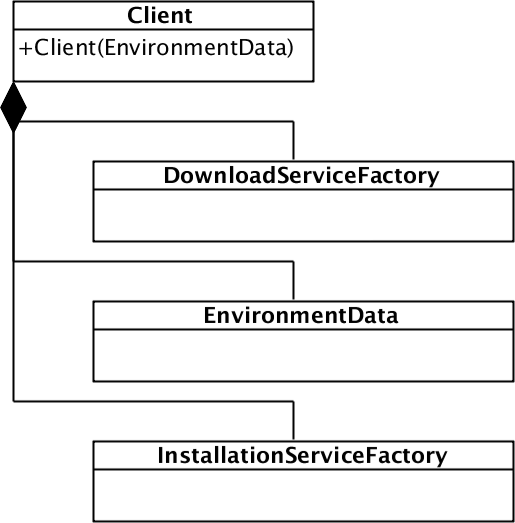
\includegraphics[bb=0 0 515 523, scale=0.50]{Client.png}
\caption{Szkic UML klasy \texttt{Client}}
\end{figure}

\subsubsection{Środowisko (ustawienia, dane instalacji)}

Jak wspomniano wcześniej, klasa \texttt{EnvironmentData} służyłaby do
przechowywania informacji związanych z tym, które programy zaktualizować i w
jaki sposób ma to zostać wykonane. Zadania te byłyby oddelegowane do instancji
klasy \texttt{ClientSettings} oraz zbioru instancji klasy
\texttt{ProgramSettings}. Powinna także tworzyć instancję klasy
\texttt{AvailabilityFilter}, która odpowiadałaby za filtrowanie wyników
zwracanych przez zapytania do repozytoriów.

Ponieważ przechowywałaby bieżący stan instalacji dla grupy zdefiniowanych
w zbiorze \texttt{ProgramSettings} programów, mogłaby służyć do zainicjowania
kilku instancji \texttt{Clienta}. Ze względu na to, że zawierałaby informacje
kluczowe do poprawnego przebiegu pobierania danych oraz instalacji, powinna
służyć programiście wyłącznie do tworzenia owych instancji.

Prawidłowym sposobem na uzyskanie instancji \texttt{EnvironmentData} powinno 
być użycie \texttt{EnvironmentDataManagera}, klasy przeznaczonej do tworzenia,
zapisywania i przywracania instancji \texttt{EnvironmentData}. Automatycznie
konwertowałaby do i z postaci dokumentów XML, przechowywanych w uprzednio
zdefiniowanej lokalizacji.

Samo położenie dokumentów z ustawieniami i danymi instalacji, wraz z pewnymi
domyślnymi wartościami mogącymi służyć utworzeniu nowej definicji instalacji
byłyby z kolei przechowywane w klasie \texttt{EnvironmentContext}.
\texttt{EnvironmentDataManager} wykorzystywałby je do zarządzania instancjami
\texttt{EnvironmentData} oraz tworzenia nowych instancji wypełnionych
domyślnymi danymi.

Klasa \texttt{ClientSettings} powinna przechowywać m.in. informacje używane
podczas tworzenia połączenia, zwiększanie uprawnień procesu oraz właściwej
instalacji. Przechowywane w niej ścieżki powinny odpowiadać ścieżkom do
prawdziwych plików i katalogów, aby zagwarantować prawidłową pracę biblioteki.

Definicja instalacji każdego programu powinna być reprezentowana przez jedną
instancję klasy \texttt{ProgramSettings}. Każdą powinna identyfikować
jednoznacznie następująca trójka:
\begin{itemize}
  \item katalog instalacji danego programu,
  \item adres repozytorium,
  \item nazwa programu w repozytorium.
\end{itemize}
Umożliwiałoby to np. posiadanie 2 instalacji współdzielących 1 katalog (np.
główna instalacja programu i jakiś moduł przechowywany w innym repozytorium),
czy też 2 różnych instalacji tego samego programu (np. w wersji rozwojowej
i produkcyjnej).

\begin{figure}[Environment]
\centering
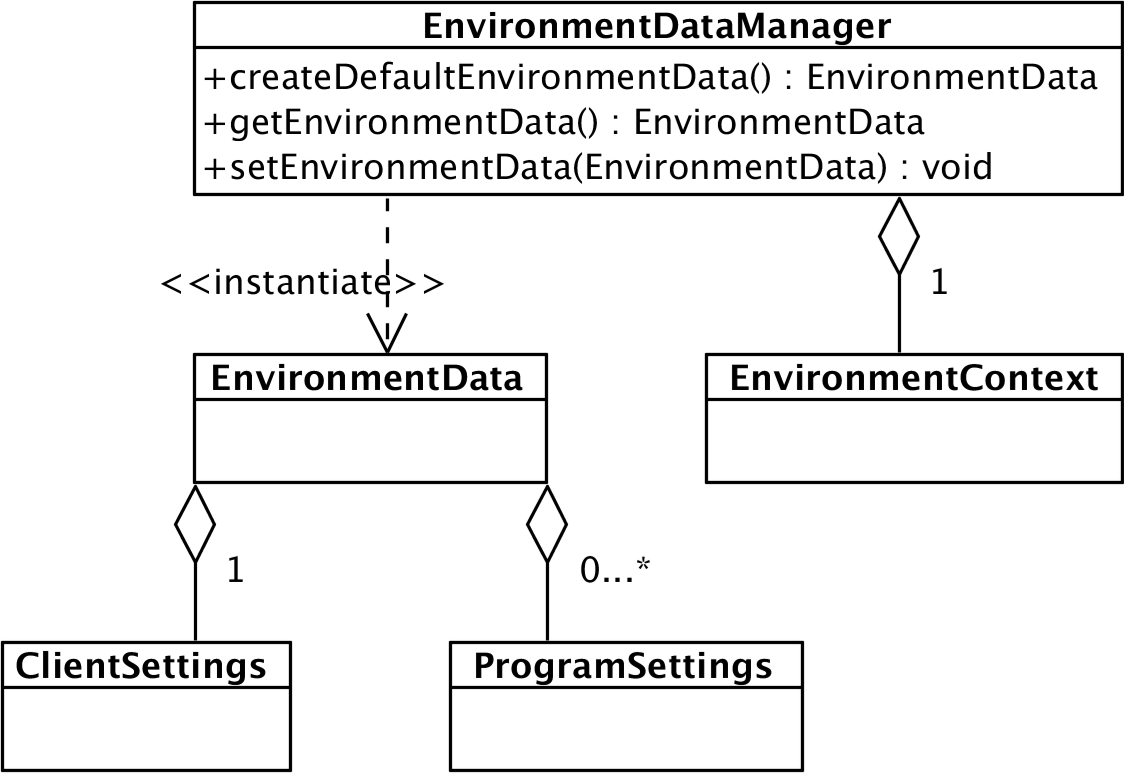
\includegraphics[bb=0 0 1124 773, scale=0.30]{Environment.png}
\caption{Szkic UML klas \texttt{EnvironmentData} i powiązanych}
\end{figure}

\subsubsection{Modele}

Niech poszczególne modele danych zostaną odwzorowane przez klasy im
odpowiadające.

Instalacje programów i pakietów zostaną więc odwzorowane przez klasy
\texttt{Program}, oraz \texttt{Package}. Klasa \texttt{Program} oprócz
posiadania własnych atrybutów opisujących i identyfikujących program,
agregowałaby również instancje klasy \texttt{Package}.

Z kolei klasa \texttt{Package} poza opisem instalacji danego pakietu, powinna
móc przechowywać zbiór dostępnych dla niej aktualizacji. Dostępne aktualizacje
byłyby w niej umieszczane jako skutek uboczny usług pobierających dane
na temat aktualizacji dla wybranych pakietów. W podobny sposób klasa Program
byłaby uzupełniana o znane błędy (instancje  klasy \texttt{BugEntry}), a klasa
\texttt{Package} o listę zmian (instancje klasy \texttt{ChangelogEntry}).

Same aktualizacje reprezentowane przez klasę \texttt{Update}, posiadałyby
przypisany do każdej z nich stan, stanowiłyby także klasę obserwowalną. Dzięki
temu możliwe byłoby łatwe zmienianie ich stanu z poziomu GUI, jak również
wyświetlanie bieżącego stanu instalacji każdej wybranej aktualizacji.

Wszystkie modele posiadałyby przeciążone metody \texttt{equals(Object)},
\texttt{hashcode()}, a także \texttt{compareTo(T)} (implementacja interfejsu
\texttt{Comparable<T>}). Wszystkie przeciążane metody zachowywałyby kontrakt
tak, aby wprowadzać poprawne relacje równoważności (do porównań) i porządku
liniowego (w celu automatycznego sortowania zbiorów przy np. wyświetlaniu
danych).

Relacje równoważności byłyby zdefiniowane następująco:
\begin{itemize}
  \item \texttt{Program} - za równe uważane są programu o tym samym katalogu,
    adresie repozytorium i nazwie na serwerze,
  \item \texttt{Package} - za równe uznajemy pakiety o tej samej nazwie i tym
    samym \texttt{Programie},
  \item \texttt{Update} - za równe uznajemy aktualizacje o tym samym numerze
    wersji, typie (wersja rozwojowa/produkcyjna) oraz pakiecie,
  \item \texttt{BugEntry} - za równe uznajemy błędy o tym samym opisie i
    programie,
  \item \texttt{ChangelogEntry} - za równe uznajemy wpisy o tym samym numerze 
    wersji i tym samym pakiecie.
\end{itemize}

\begin{figure}[!ht]
\centering
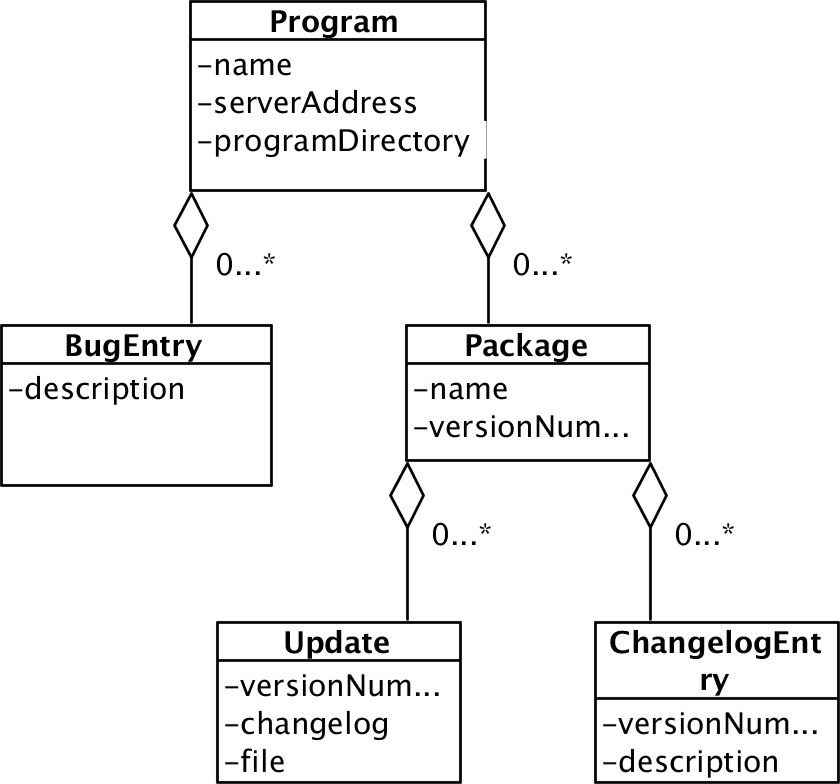
\includegraphics[bb=0 0 840 784, scale=0.35]{Models.png}
\caption{Szkic UML modeli}
\end{figure}

\subsubsection{Agregowane usługi pobierania (wiele pobrań z przetwarzaniem wyników)}

Klasy \texttt{AggregatedDownloadService} powinny wykonywać kilka pobrań z
wykorzystaniem puli wątków. Zadanie jest uznawane za zakończone, jeśli
wszystkie poszczególne zadania pobierania zastały zakończone, bez względu
na ich wynik.

Powinny również tworzyć instancje \texttt{AggregatedNotifiers}, które będą
Obserwowalnymi Obserwatorami \cite{OBSERWATOR} wszystkich zadań pobierania,
zarządzanymi przez konkretną usługę. Mogą być później wykorzystane do
zbierania bieżących informacji o stanie pobierania.

Każda klasa \texttt{AggregatedDownloadService} powinna implementować również
metodę agregującą wyniki wszystkich procesów, czy to poprzez zwracanie
kolekcji zawierającej wyniki wszystkich pobierań, czy też poprzez bardziej
wyrachowane zachowanie takie jak aktualizowanie pól modeli danych.
Przykładowo, po pobraniu informacji na temat aktualizacji, modele pakietów
powinny zostać zaktualizowane o listy dostępnych aktualizacji. Podobnie
aktualizowane byłyby pola z informacjami z listy zmian oraz znanymi błędami.

Usługi powinny być tworzone przez fabrykę \texttt{DownloadServiceFactory},
zapewniającą poprawną inicjalizację każdej instancji
\cite{FABRYKA_ABSTRAKCYJNA}.

\begin{figure}[!ht]
\centering
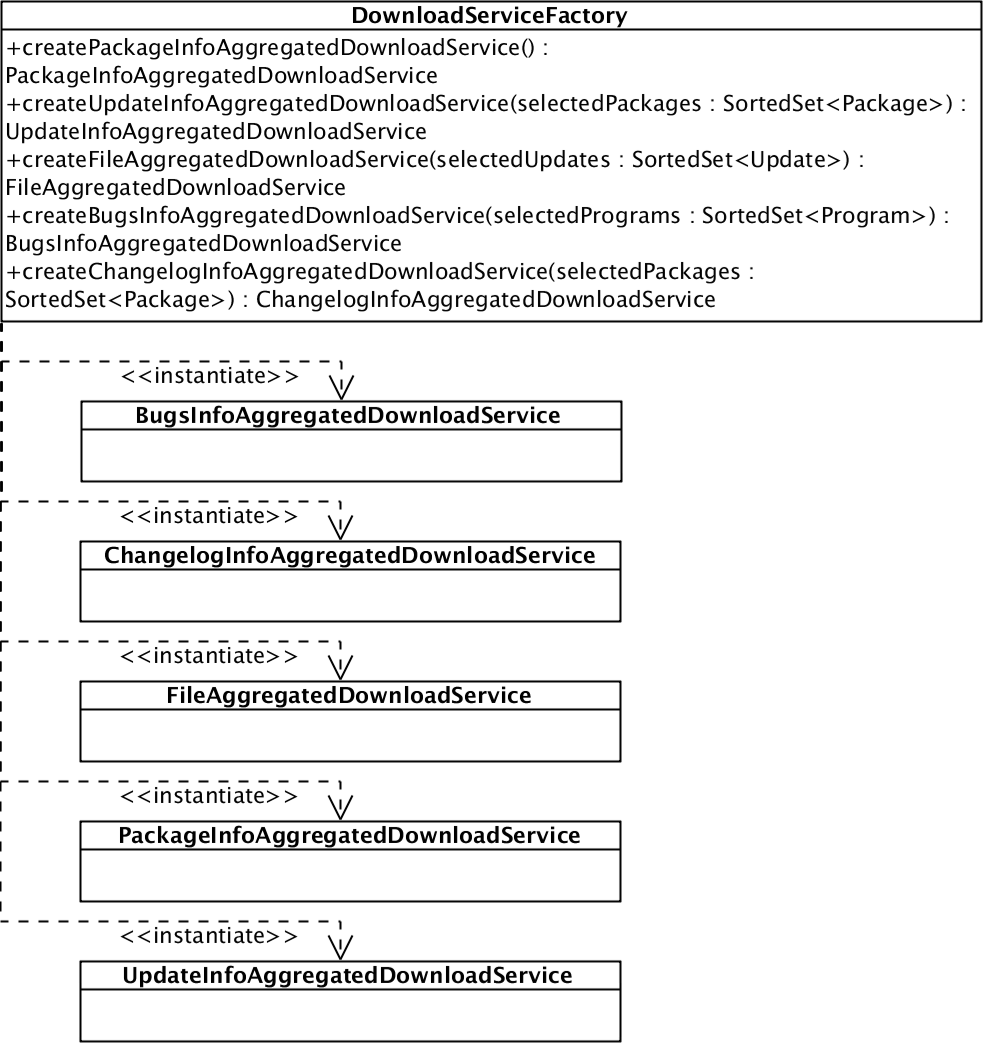
\includegraphics[bb=0 0 983 1043, scale=0.40]{AggregatedDownloadServices.png}
\caption{Szkic UML klas \texttt{AggregatedDownloadService}}
\end{figure}

\subsubsection{Działania zależne od platformy}

Powinien zostać zdefiniowany sposób wykonywania zadań zależnych od danego
systemu, który pozwalałby w czasie uruchomienia wybrać odpowiednią
implementację. Jednym z najprostszych rozwiązań jest zastosowanie wzorca
Strategii \cite{STRATEGIA}, która będzie udostępniać implementacje 
interfejsów  opisujących rzeczone czynności, która byłaby dostępna poprzez 
pewną Fabrykę Abstrakcyjną.

Java umożliwia stworzenie strategii przy pomocy typu wyliczeniowego - jego
instancje są naturalnymi singletonami \cite{SINGLETON}, zaś sam język pozwala
dodawać do nich pola i metody \cite{DODAWANIE_METOD_ENUM}. Mogą one być
zainicjowane przy pomocy przeciążonych konstruktorów. Rolę fabryki mogłaby
pełnić statyczna metoda klasy.

Możemy przyjąć, że naszym typem wyliczeniowym byłaby klasa
\texttt{EOperatingSystem}, posiadająca metody, zwracające instancje
\texttt{IProcessKillera} i \texttt{IProcessExecutora}.

Niech \texttt{IProcessExecutor} będzie interfejsem stanowiącym bazę dla
wszystkich implementacji tworzących nowe procesy poza maszyną wirtualną Javy.
Jako, że sama baza klas JDK udostępnia środki do wywołania procesów
działających natywnie, można wydzielić pewną część wspólną wszystkich
implementacji, np. klasę abstrakcyjną, realizującą to zadanie. Oddzielna
implementacja sprowadzałaby się do napisania kodu odpowiedzialnego za
uzyskanie uprawnień superużytkownika na danej platformie.

Kończenie działania procesu nieutworzonego z użyciem klasy \texttt{Process}
jest niemożliwe bez odwołania się do narzędzi udostępnionych przez dany system
operacyjny. Sama Java umożliwia wyłącznie zakończenie działania procesu
bezpośrednio przez nią uruchomionego, do którego mamy dostęp poprzez instancję
klasy \texttt{Process} - jego procesy potomne, jak również inne, dla których
nie dysponujemy instancją klasy \texttt{Process} muszą zostać zamknięte w
natywny dla danego systemu sposób \cite{JAVA_TERMINACJA}.

Poszczególne implementacje mogłyby więc wykorzystywać interfejs
\texttt{IProcessKiller}, używając do zakończenia procesów narzędzia
udostępnione bezpośrednio przez dany system operacyjny.

\begin{figure}[!ht]
\centering
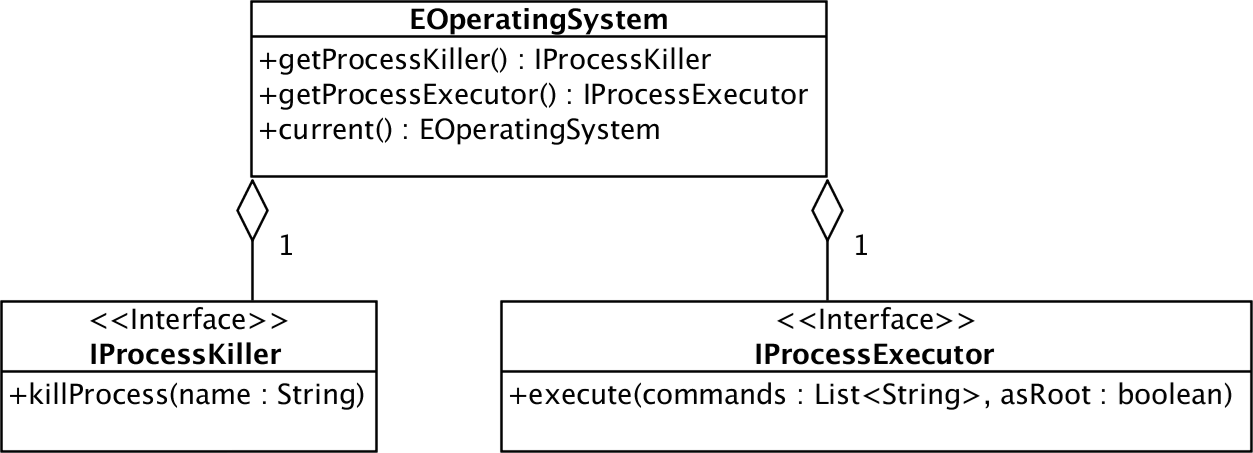
\includegraphics[bb=0 0 1253 453, scale=0.30]{OperatingSystem.png}
\caption{Szkic UML klas obsługujących operacje zależne od platformy}
\end{figure}

\subsubsection{Instalator (plik wykonywalny)}

Właściwa instalacja powinna być wykonywana przez zewnętrzny plik wykonywalny
JAR - zapewnia to przenośność kodu, tak długo, jak tylko zaimplementowane
zostaną interfejsy do uruchamiania procesów z podniesionymi uprawnieniami - 
ponieważ nie możemy wymagać od użytkownika, aby uruchamiał klienta z takowymi
(jest to niebezpieczne, a często również niemożliwe do wykonania), zamiast
tego klient zostanie uruchomiony z normalnym poziomem uprawnień, zaś o
ewentualne zwiększenie uprawnień użytkownik zostanie poproszony przez
specjalne okno dialogowe tuż przed właściwą instalacją aktualizacji.

Sam instalator najpierw wykonywać będzie kopię bezpieczeństwa, a następnie 
dokona instalacji aktualizacji według jednej z trzech zdefiniowanych w
wymaganiach funkcjonalnych strategii.

Wynik zostanie zwrócony na standardowe wyjście i/lub wyjście błędów
w zależności od powodzenia danej operacji. Przyjęty zostanie pewien format
wyjścia, aby możliwe było parsowanie wyników przez bibliotekę i aktualizowanie
informacji na temat bieżącego stanu instalacji.

\begin{figure}[!ht]
\centering
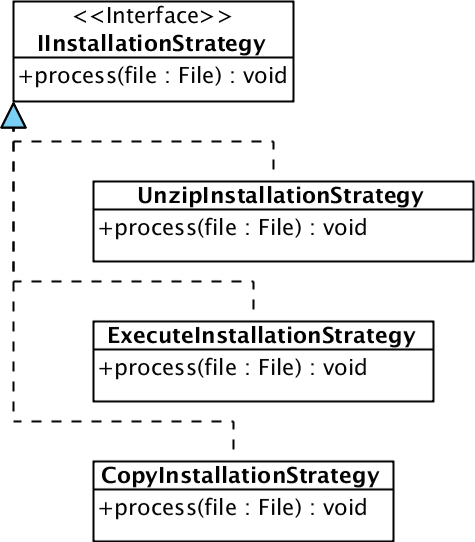
\includegraphics[bb=0 0 475 542, scale=0.50]{Installer.png}
\caption{Szkic UML klas bezpośrednio obsługujących instalację}
\end{figure}

\subsubsection{Usługi instalacji (uruchamianie instalacji z poziomu biblioteki)}

Przygotowanie polecenie wykonującego aktualizację i parsowanie rezultatów jest
złożonym zadaniem, dlatego też powinna zostać utworzona specjalna usługa
przeznaczona wyłącznie w tym celu (Fasada \cite{FASADA}).

Dla spójności nazwijmy ją \texttt{AggregatedInstallationService}. Podobnie jak
w przypadku usług \texttt{AggregatedDownloadService} będzie ona wykonywała
wiele operacji, a następnie przetwarzała ich wyniki do odpowiedniej postaci.

Powinna ona robić użytek z implementacji \texttt{IProcessKiller} i
\texttt{IProcessExecutor} do zakończenia działających programów i dokonania
instalacji.

O tym, które aktualizacje będą wybrane do instalacji niech decyduje stan
aktualizacji: programista będzie mógł wybrać czy są one wybrane do instalacji
czy też nie. Instalacje już zainstalowane, będą traktowane jak niewybrane,
zaś te, które anulowano lub zakończyły się niepowodzeniem będą traktowane jak
wybrane do instalacji, o ile programista nie zmieni ich stanu na inny - fakt
anulowanej bądź zakończonej niepowodzeniem instalacji świadczy o uprzednim
wyborze programisty, który z jakiś powodów nie mógł zostać wykonany przez
program.

Skonfigurowane instancje \texttt{AggregatedInstallationService} powinny być
tworzone przez fabrykę \texttt{InstallationServiceFactory}.

\begin{figure}[!ht]
\centering
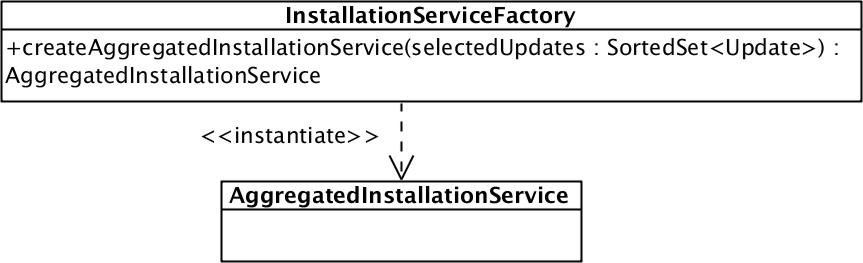
\includegraphics[bb=0 0 863 263, scale=0.50]{Installation.png}
\caption{Szkic UML klas pośrednio obsługujących instalację}
\end{figure}


\subsection{Diagramy sekwencji}

\subsubsection{Pobieranie aktualizacji}

Pobieranie aktualizacji zaczyna się od stworzenia obiektu
\texttt{AggragatedPackageInfoDownloadService}, który pobierze informacje na
temat dostępnych pakietów (oraz programów). Odbywa się to przy pomocy
instancji klasy \texttt{Client}.

Po pobraniu programów, programista tworzy zbiór pakietów dla których chce
pobrać informacje o aktualizacjach. Następnie tworzy dla nich instancję
\texttt{AggregatedUpdateInfoDownloadService}, która zajmie się pobraniem
danych.

W końcu dla wybranych aktualizacji utworzona zostaje instancja klasy
\texttt{AggregatedFileDownloadService}, która pobierze pliki i umieści je w
instancjach modelu \texttt{Update}.

\begin{figure}[!ht]
\centering
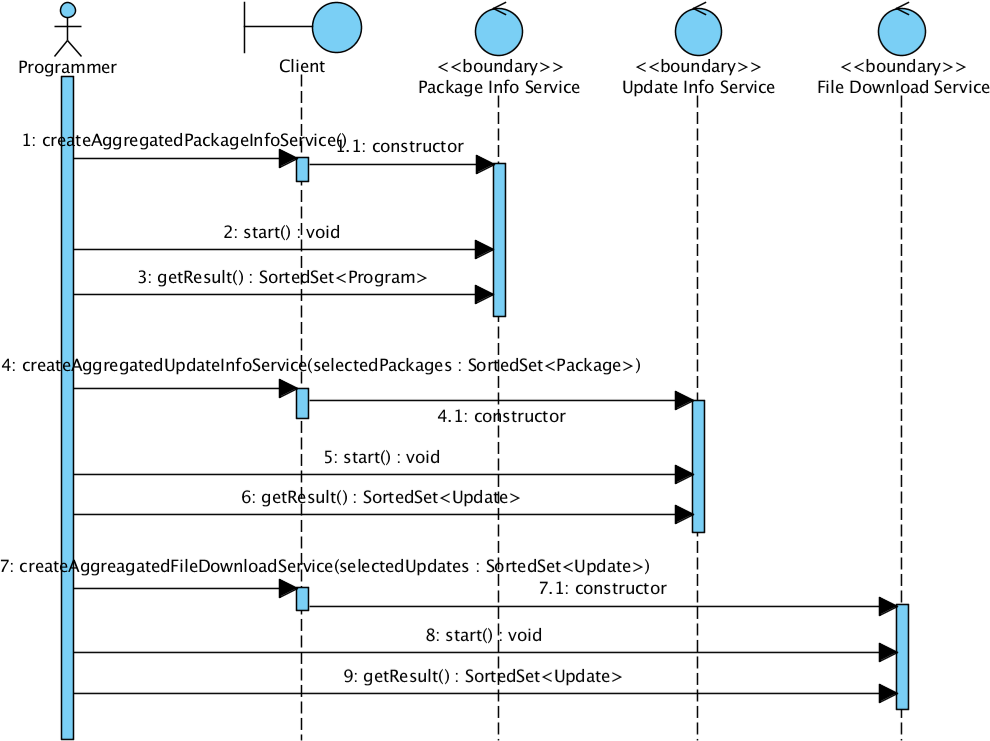
\includegraphics[bb=0 0 990 741, scale=0.40]{UpdateSequence.png}
\caption{Diagram obrazujący proces pobierania aktualizacji}
\end{figure}

\subsubsection{Pobieranie list błędów}

Aby pobrać listę błędów konieczne jest posiadanie zbioru dostępnych w
repozytoriach programów i wybranie z nich tych, które nas interesują.
Wówczas informacje o błędach mogą zostać pobrane przy pomocy instancji
\texttt{AggregatedBugsInfoDownloadService}.

Po pobraniu listy błędów zostaną umieszczone w instancjach modelu
\texttt{Program}.

\begin{figure}[!ht]
\centering
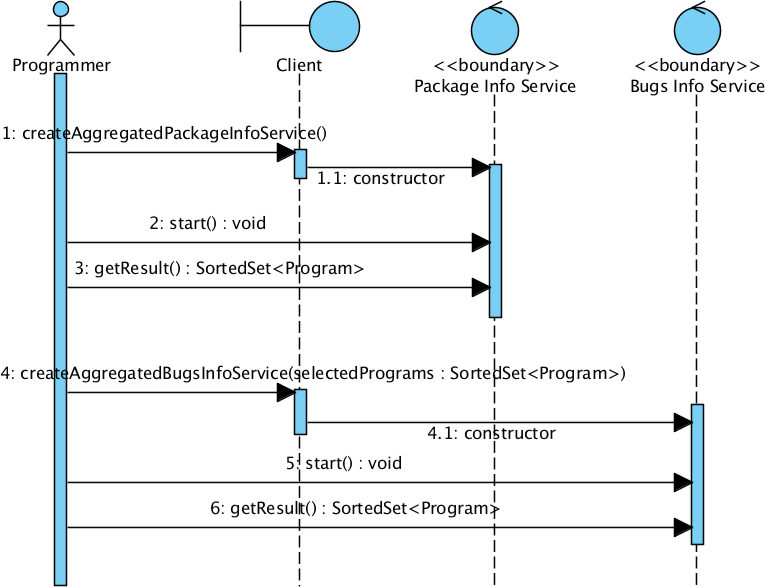
\includegraphics[bb=0 0 765 587, scale=0.40]{BugsSequence.png}
\caption{Diagram obrazujący proces pobierania znanych błędów programów}
\end{figure}

\subsubsection{Pobieranie list zmian}

Aby pobrać listę zmian konieczne jest posiadanie zbioru dostępnych w
repozytoriach programów i wybranie z nich tych pakietów, które nas interesują.
Wówczas informacje mogą zostać pobrane przy pomocy instancji
\texttt{AggregatedChangelogInfoDownloadService}.

Po pobraniu listy zmian zostaną umieszczone w instancjach modelu
\texttt{Package}.

\begin{figure}[!ht]
\centering
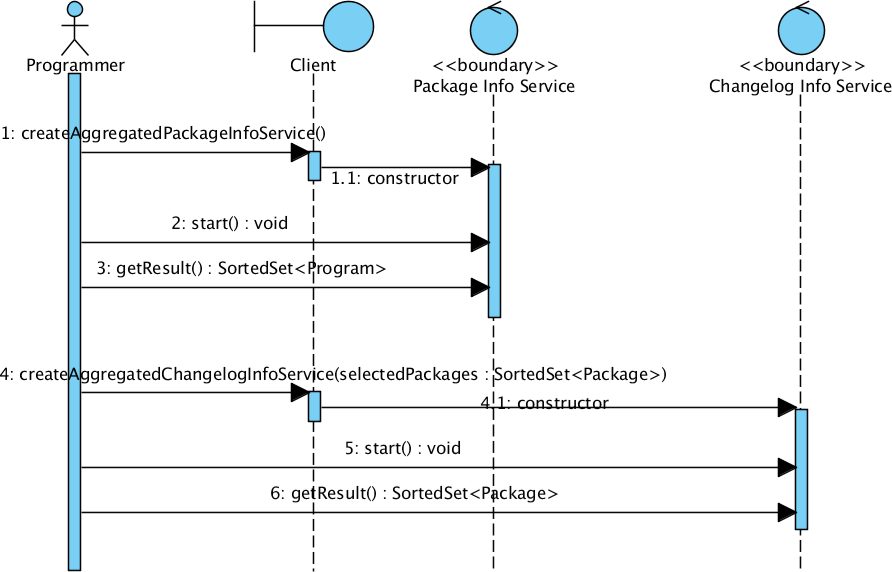
\includegraphics[bb=0 0 892 572, scale=0.40]{ChangelogSequence.png}
\caption{Diagram obrazujący proces pobierania list zmian pakietów}
\end{figure}

\newpage

%%%%%%%%%%%%%%%%%%%%%%%%%%%%%%%%%%%%%%%%%%%%%%%%%%%%%%%%%%%%%%%%%%%%%%%%%%%%%%
%%%%%%%%%%%%%%%%%%%%%%%%%%%%%% IMPLEMENTATION %%%%%%%%%%%%%%%%%%%%%%%%%%%%%%%%
%%%%%%%%%%%%%%%%%%%%%%%%%%%%%%%%%%%%%%%%%%%%%%%%%%%%%%%%%%%%%%%%%%%%%%%%%%%%%%

\section{Implementacja}


\subsection{Opis technologii}

Ze względu na wymagania niefunkcjonalne zarówno biblioteka jak i GUI zostały
wykonane przy pomocy Javy SE 7. Wyjątek stanowi program do zdobywania
uprawnień administratora na systemach z rodziny Windows, napisany w języku
C\#.

Testy jednostkowe zostały napisane przy pomocy biblioteki FEST Assertions
\cite{FEST_ASSERTIONS}, zaś klasy mockujące przy pomocy biblioteki Mockito
\cite{MOCKITO}.

W kodzie biblioteki niektóre zadania zrealizowano z pomocą biblioteki
Guava \cite{GUAVA}. Do parsowania danych XML pobranych z serwera służy
biblioteka Jaxen \cite{JAXEN}.
\\

Wszystkie wykorzystane biblioteki rozpowszechniane są na zasadach wolnego oprogramowania.


\subsection{Objaśnienie kodu źródłowego}

Zadania zależne od platformy systemowej zostały umieszczone w projekcie
\texttt{AutoUpdaterSystem}, rdzeń biblioteki w projekcie
\texttt{AutoUpdaterLibrary}, klasy zawierające informacje wspólne dla
biblioteki i instalatora w projekcie \texttt{AutoUpdaterCommons}, sam zaś
instalator w projekcie \texttt{AutoUpdaterInstaller}.

Przykładowy graficzny interfejs użytkownika został umieszczony w projekcie
\texttt{AutoUpdaterGUI}.

Wszystkie wymienione projekty zawierają plik \path!build.xml! budujący pliki
JAR przy pomocy programu Ant i umieszczający je wraz z wymaganymi bibliotekami
w katalogu \path!AutoUpdater!.

Programy do podnoszenia uprawnień na platformie Windows znajdują się
w projektach \texttt{UACHandler} i \texttt{UACProvider}.

Wszystkie klasy i najważniejsze metody biblioteki zostały opisane przez
dokumentację Javadoc, którą można znaleźć w katalogu wraz projektami.

Sposób wykorzystania każdej klasy, która jest przeznaczona do bezpośredniego
wykorzystania przez programistę został opisany w dokumentacji.

W podanych przykładach kodu źródłowego nie zawarto dokumentacji Javadoc.

\subsubsection{Wykorzystane wzorce projektowe i elementy języka}

Wśród częściej wykorzystywanych elementów języka należy wymienić wykorzystanie
metody \texttt{equals(Object)} do porównywania dwóch obiektów. Dzięki jej
przeciążeniu możliwe było dokonywanie porównań, wykorzystywanie operacji na
kolekcjach, i wyszukiwanie wymaganych obiektów przy użyciu bibliotek
systemowych, bądź biblioteki Guava opartej na standardowych mechanizmach
Javy. Analogicznie ma się sprawa z metodą \texttt{hashcode()} oraz
\texttt{compareTo(T)} interfejsu \texttt{Comparable<T>}.

Uczyniono również użytek z możliwości jakie daje typ wyliczeniowy -
dodawanie pól prywatnych, inicjowanie ich przez przeciążony konstruktor,
dodawanie własnych metod \cite{DODAWANIE_METOD_ENUM}, czy zastępowanie
konstrukcji \texttt{swich} poprzez wywołanie metody typu wyliczeniowego tam,
gdzie to możliwe.

Kod jest sterowany wyjątkami, dzięki czemu zwiększono jego czytelność i
pozwolono programiście na przejrzystą obsługę błędów.

Jednym z wykorzystanych wzorców projektowych jest metoda wytwórcza
\cite{METODA_WYTWORCZA}. Użyto jej do wyekstraktowania logiki m.in. strategii
pobierania z klas \texttt{AbstractDownloadService} (oddelegowanej do
implementacji klasy \texttt{IPostDownloadStrategy}), zaś w klasie
\texttt{AggregatedDownloadService} wykorzystanej do utworzenia instancji
notyfikatora.

Metody te następnie wykorzystano w metodach szablonowych
\cite{METODA_SZABLONOWA} odpowiednich klas.

Zarówno usługi pobierania jak i instalacji tworzone są przy użyciu Fabryk
\cite{FABRYKA_ABSTRAKCYJNA}. Dzięki temu cała procedura inicjalizacji usług
mogła zostać ukryta przed programistą, który musi tylko wywołać metodę start()
na gotowym do użycia obiekcie. Same fabryki wkomponowano \cite{KOMPOZYT} w
klasę \texttt{Client}.

Wewnątrz biblioteki do tworzenia instancji  modeli wykorzystano wzorzec
Budowniczego \cite{BUDOWNICZY}. Pozwoliło to uniknąć tworzenia dużej ilości
rozbudowanych konstruktorów, które zaciemniałyby kod i utrudniały jego
utrzymanie.

Do uruchamiania oraz terminacji procesów wykorzystano wzorzec Strategii
\cite{STRATEGIA} - o wyborze strategii programista może zadecydować sam, lub
też pobrać instancję opisującą bieżącą platformę sprzętową poprzez wywołanie
\texttt{EOperatingSystem.current()}
\footnote{pakiet \texttt{com.autoupdater.system} w projekcie
AutoUpdaterSystem}, z której uzyska interesującą go implementację
\texttt{IProcessKiller} \footnote{pakiet
\texttt{com.autoupdater.system.process.killers} w projekcie AutoUpdaterSystem}
lub \texttt{IProcessExecutor} \footnote{pakiet
\texttt{com.autoupdater.system.process.executors}
w projekcie AutoUpdaterSystem}.

\subsubsection{Proces pobierania danych z serwera}

Bezpośrednio za pobieranie danych z serwera odpowiadają klasy rozszerzające
\texttt{AbstractDownladRunnable} \footnote{pakiet 
\texttt{com.autoupdater.client.download.runnables} w 
projekcie AutoUpdaterLibrary}. Jest to klasa generyczna, w której
parametrem jest typ zwracanego rezultatu deklarująca chronioną metodę
abstrakcyjną \texttt{getPostDownladStrategy()}. Ma ona za zadanie zwracać
implementację interfejsu \texttt{IPostDownladStrategy} \footnote{pakiet
\texttt{com.autoupdater.client.download.runnables.post.download.strategies} w
projekcie AutoUpdaterLibrary}, odpowiadającą za
operowanie na pobranych danych - w zależności od potrzeb może być to
przetworzenie XMLa przez konkretny parser, bądź zapisanie danych do pliku - a
następnie zwrócenie wyniku operacji.

Za uruchomienie instancji \texttt{AbstractDownloadRunnable} odpowiadają
rozszerzenia klasy \texttt{AbstractDownloadService} \footnote{pakiet
\texttt{com.autoupdater.client.download.services} w projekcie
AutoUpdaterLibrary}. Inicjują one odpowiednią instancję
\texttt{AbstractDownloadRunnable} i zwracają jej wynik po zakończeniu
pobierania. Do utworzenia wymagają adresu z którego mają pobrać dane, który to
adres przekazują instancji \texttt{Runnable}. Są to obserwowalne klasy,
regularnie wysyłające komunikaty na temat bieżącego stanu pobierania.

Do grupowania powiązanych usług służą instancje
\texttt{AbstractAggregatedDownloadService} \footnote{pakiet
\texttt{com.autoupdater.client.download.aggregated.services} w projekcie
AutoUpdaterLibrary}. Uruchamiają one poszczególne usługi przy pomocy puli
wątków, aby ograniczyć zużycie zasobów wykorzystywanych przez aplikację w
danej chwili. Udostępniają instancje klasy
\texttt{AbstractAggregatedNotification} \footnote{pakiet
\texttt{com.autoupdater.client.download.aggregated.notifiers} w projekcie
AutoUpdaterLibrary} wysyłające komunikaty odebrane od wszystkich zagregowanych
usług. Dodatkowo deklaruje metodę \texttt{getResults()}, która próbuje pobrać
wyniki wszystkich pobrań i przetwarza je do żądanej postaci.

Dla wygody programistów korzystających z biblioteki zadaniem odpowiedniego
zainicjowania zagregowanych usług pobierania zajmuje się klasa
\texttt{DownloadServiceFactory} \footnote{pakiet
\texttt{com.autoupdater.client.download} w projekcie AutoUpdaterLibrary}
wkomponowana w klasę \texttt{Client} \footnote{pakiet
\texttt{com.autoupdater.client} w projekcie AutoUpdaterLibrary}.

\subsubsection{Pobieranie informacji na temat postępów}

Każda zagregowana usługa pobierania posiada instancję klasy
\texttt{AbstractNotifier} \footnote{pakiet
\texttt{com.autoupdater.client.utils.services.notifier} w projekcie
AutoUpdaterLibrary}. Gromadzi ona informacje ze wszystkich usług jakie
są zarządzane przez pulę wątków klasy \texttt{AbstractAggregatedService}.
Możliwe jest obserwowanie jej bezpośrednio, dzięki czemu obserwator otrzyma
informacje o postępach wszystkich pobierań jak również o całkowitym
zakończeniu procesu pobierania.

Ponieważ wymagałoby to tworzenia rozległego kodu oddelegowującego otrzymane
wiadomości do odpowiednich instrukcji, możliwe jest zamiast tego wykorzystanie
metody \texttt{getService(AdditionalMessage)}, wykorzystującej powiązanie
pomiędzy usługą a pewnym dodatkowym parametrem - zazwyczaj instancją modelu
wykorzystanego do jej utworzenia (np. model \texttt{Update} pomaga w
utworzeniu usług pobierania plików dla aktualizacji, a model \texttt{Package}
w utworzeniu usług zdobywających informacje o dostępnych aktualizacjach
\footnote{modele znajdują się w pakiecie
\texttt{com.autoupdater.client.models} w projekcie AutoUpdaterLibrary}).
Ponieważ każda usługa pobierania jest obserwowalna, informacje na temat
postępów możemy otrzymywać bezpośrednio z niej.

Nieco inaczej wygląda pobieranie informacji na temat postępów instalacji.
Instancja \texttt{InstallationNotifier} \footnote{pakiet
\texttt{com.autoupdater.client.installation.notifiers} w projekcie
AutoUpdaterLibrary} udostępnia informacje na temat postępu procesu jako
całości, zaś postęp konkretnej aktualizacji jest dostępny od razu w modelu
\texttt{Update} - każda jego instancja jest obserwowalnym obiektem wysyłającym
wiadomość o każdej zmianie swojego statusu. W dowolnej chwili możemy pobrać tą
informację poprzez metodę \texttt{getUpdateStatus()}.

\subsubsection{Współdzielenie informacji między biblioteką a instalatorem}

Biblioteka oraz instalator posiadają wspólne niektóre klasy opisujące
sposób ich komunikacji - są to formaty komunikatów wysyłanych przez instalator
na wyjście, a odczytywanych przez odpowiedni parser biblioteki.

Umieszczone są one w osobnym projekcie eksportowanym do pliku .jar, dzięki
czemu, po umieszczeniu go w \texttt{ClassPathu} \footnote{Definiowana przy
uruchomieniu maszyny wirtualnej ścieżka lub ścieżki, które mając być
przeszukane pod kątem obecności plików .class lub .jar} tak klienta jak i
instalatora, oba programy operują na tych samych danych. Dzięki temu
utrzymywanie osobnego kodu generującego wyniki i kodu odczytujące je zostało
ograniczone do minimum.

\begin{lstlisting}[language=Java, frame=lines, numberstyle=\tiny,
stepnumber=5, caption=Typ wyliczeniowy opisujący etap instalacji., firstnumber=1]
package com.autoupdater.commons.messages;

public enum EInstallerMessage {
    PREPARING_INSTALLATION("Preparing installation..."),
    BACKUP_STARTED("Backup started..."),
    BACKUP_FINISHED("Backup finished"),
    BACKUP_FAILED("Backup failed"),
    INSTALLATION_STARTED("Installation started..."),
    POST_INSTALLATION_COMMAND_EXECUTION("Executing post-installation commands..."),
    POST_INSTALLATION_COMMAND_EXECUTION_FINISHED("Post-installation command execution failed"),
    POST_INSTALLATION_COMMAND_EXECUTION_FAILED("Post-installation command execution failed"),
    INSTALLATION_FINISHED("Installation finished"),
    INSTALLATION_FAILED("Installation failed");

    private String message;

    private EInstallerMessage(String message) {
        this.message = message;
    }

    public String getMessage() {
        return message;
    }

    @Override
    public String toString() {
        return message;
    }
}
\end{lstlisting}

Przykładowo, klasa \texttt{EInstallerMessage} \footnote{pakiet
\texttt{com.autoupdater.commons.message} w projekcie AutoUpdaterCommons}
zawiera wiadomości zwracane przez instalator na danym etapie instalacji.
Biblioteka jest w stanie zamienić wiadomość z powrotem na typ wyliczeniowy i
na jego podstawie przeprowadzić odpowiednią operację.

\subsubsection{Implementacja zadań zależnych od systemu operacyjnego}

Zadania zależne od danego systemu - terminacja i tworzenie procesów zostały
zrealizowane jako implementacje interfejsów \texttt{IProcessKiller} oraz
\texttt{IProcessExecutor} zwracane przez odpowiednie instancje klasy
\texttt{EOperatingSystem}. Sama instancja dla bieżącego systemu może być
pobrana przy pomocy metody statycznej \texttt{current()}.

\begin{lstlisting}[language=Java, frame=lines, numberstyle=\tiny,
stepnumber=5, caption=Implementacja \texttt{EOperatingSystem}., firstnumber=1]
package com.autoupdater.system;

...

public enum EOperatingSystem {
    WINDOWS("Windows", OperatingSystemConfiguration.WINDOWS_LOCAL_APP_DATA,
            new WindowsProcessExecutor(), new WindowsProcessKiller(), "tasklist"),

    LINUX("Linux", OperatingSystemConfiguration.LINUX_LOCAL_APP_DATA, new LinuxProcessExecutor(),
            new LinuxProcessKiller(), "echo \"content\"");

    ...

    public String getLocalAppData() {
        return localAppData;
    }

    public IProcessExecutor getProcessExecutor() {
        return processExecutor;
    }

    public IProcessKiller getProcessKiller() {
        return processKiller;
    }

    ...

    public static EOperatingSystem current() {
        return current;
    }
}
\end{lstlisting}

Implementacje interfejsu \texttt{IProcessKiller} są względnie proste -
polegają one na wywołaniu metod, które sprawdzają czy proces o danej nazwie
istnieje, a jeśli tak to wysyłają sygnał \texttt{TERM}/\texttt{KILL}, w
zależności od potrzeb.

W przypadku systemów Linux komenda \texttt{kill PID} zakończy proces o id
,,PID''. Jeśli uruchomiona zostanie z parametrem \texttt{TERM} program do
programu zostanie wysłany sygnał terminacji, które może zostać obsłużony
przez np. wyświetlenie okna dialogowego o treści ,,Czy chcesz zapisać zmiany
przed zamknięciem?''. Przedstawiona implementacja będzie próbować zakończyć
program w ten sposób - dopiero jeśli o zawiedzie, odwoła się do zabicia
procesu siłą \cite{LINUX_TERMINACJA}.

Ponieważ polecenie terminujące działa asynchronicznie, konieczne jest
odczekanie pewnej chwili na upewnienie się, że proces został zakończony.
W przypadku porażki, możliwe jest podjęcie kolejnych prób. Dopiero jeśli
wszystkie zawiodą zwracany jest wyjątek.

\begin{lstlisting}[language=Java, frame=lines, numberstyle=\tiny, stepnumber=5, caption=Implementacja \texttt{LinuxProcessKiller}., firstnumber=1]
package com.autoupdater.system.process.killers;

...

public class LinuxProcessKiller implements IProcessKiller {
    @Override
    public void killProcess(String programName) throws IOException, InterruptedException,
            ProcessKillerException {
        int attempts = 0;

        if (!isProgramRunning(programName))
            return;

        for (attempts = 0; attempts < ProcessKillerConfiguration.HOW_MANY_ATTEMPTS_BEFORE_FAIL; attempts++) {
            for (String pid : getPID(programName))
                if (!askToDieGracefully(pid)) {
                    killAllResistants(pid);
                }

            if (!isProgramRunning(programName))
                return;

            Thread.sleep(ProcessKillerConfiguration.HOW_MANY_SECONDS_BETWEEN_ATTEMPTS * 1000);
        }

        throw new ProcessKillerException("Couldn't kill process - "
                + ProcessKillerConfiguration.HOW_MANY_ATTEMPTS_BEFORE_FAIL + " attempts failed");
    }

    private boolean askToDieGracefully(String pid) throws IOException, InterruptedException {
        return new ProcessBuilder("kill", "-TERM", pid).start().waitFor() == 0;
    }

    private void killAllResistants(String pid) throws IOException, InterruptedException,
            ProcessKillerException {
        Process process = new ProcessBuilder("kill", pid).start();

        BufferedReader reader = new BufferedReader(new InputStreamReader(process.getErrorStream()));

        int errorCode = process.waitFor();

        if (errorCode != 0) {
            String message = reader.readLine();
            throw new ProcessKillerException(
                    message != null && message.length() > 7 ? message.substring(7, message.length())
                            : "Couldn't kill process \"" + pid + "\"");
        }
    }

    private boolean isProgramRunning(String programName) throws IOException, InterruptedException {
        Process process = new ProcessBuilder("ps", "-ef").start();

        BufferedReader outputReader = new BufferedReader(new InputStreamReader(
                process.getInputStream()));

        process.waitFor();

        String outputMessage;
        while ((outputMessage = outputReader.readLine()) != null) {
            if (outputMessage.contains(programName))
                return true;
        }

        return false;
    }

    private List<String> getPID(String programName) throws IOException {
        Process process = new ProcessBuilder(new String[] { "ps", "-ef" }).start();

        BufferedReader reader = new BufferedReader(new InputStreamReader(process.getInputStream()));

        List<String> pids = new ArrayList<String>();

        Pattern pattern = Pattern.compile("^\\S+\\s+(\\d+).+" + Pattern.quote(programName));

        String result;
        while ((result = reader.readLine()) != null) {
            Matcher matcher = pattern.matcher(result);
            if (matcher.find())
                pids.add(matcher.group(1));
        }

        return pids;
    }
}
\end{lstlisting}

Działanie Windowsowej implementacji jest analogiczne. Główna różnica polega na
tym, że komenda \texttt{TASKKILL /IM PROGRAM\_NAME} jest w stanie zakończyć
wszystkie procesy o nazwie programu ,,PROGRAM\_NAME'', przez co nie jest
konieczne ręczne zakończenie każdego procesu z osobna
\cite{WINDOWS_TERMINACJA}.

Bardziej złożone jest działanie implementacji \texttt{IProcessExecutor}. W
zależności od systemu operacyjnego, wymagane jest użycie odmiennych programów
pomocniczych, umożliwiających wykonanie kilku procesów z uprawnieniami
użytkownika, przy co najwyżej jednej prośbie o uprawnienia.

Na większości dystrybucji systemu Linux obecny jest pakiet ,,polkit''
umożliwiający łatwe uzyskanie uprawnień przy pomocy okna z prośbą o
uprawnienia. Dokonywane jest to poprzez wywołanie polecenia \texttt{pkexec
PROGRAM [ARGUMENTY\_ODDZIELONE\_SPACJĄ]} \cite{LINUX_UPRAWNIENIA}.

Polecenie to uruchamia jednak tylko jeden program. Jeśli zamierzamy wykonać
więcej niż jedno polecenie na raz, koniczne jest każdorazowe generowanie
skryptu je wywołującego lub stworzenie programu, który zajmowałby się
wywoływaniem właściwych poleceń. W tym przypadku zastosowano drugie
rozwiązanie.

\begin{lstlisting}[language=Java, frame=lines, numberstyle=\tiny, stepnumber=5, caption=Implementacja \texttt{LinuxProcessExecutor}., firstnumber=1]
package com.autoupdater.system.process.executors;

...

public class LinuxProcessExecutor extends AbstractProcessExecutor {
    @Override
    protected List<String[]> rootCommand(String uacHandler, List<String[]> commands) {
        List<String> command = new ArrayList<String>();
        command.add("pkexec");
        command.addAll(MultiCaller.prepareCommand(commands));
        return Commands.convertSingleCommand(command);
    }
}
\end{lstlisting}

Klasa pomocnicza \texttt{MultiCaller} \footnote{pakiet
\texttt{com.autoupdater.system.process.executors} w projekcie
AutoUpdaterSystem} posiada metodę statyczną \texttt{main(String[])} traktującą
wszystkie przesłane do niej argumenty, jako polecenia do wywołania. Posiada
również metodę pozwalającą wygenerować polecenie, które ją uruchomi. Wywołuje
ono metodę \texttt{main} na podstawie położenia klasy, przekazując do nowej
instancji maszyny wirtualnej bieżącą wartość zmiennej \texttt{ClassPath},
dzięki czemu nowa instancja ma dostęp do wszystkich klas do jakich miał dostęp
tworzący wywołanie program.

\begin{lstlisting}[language=Java, frame=lines, numberstyle=\tiny, stepnumber=5, caption=Implementacja \texttt{MultiCaller}., firstnumber=1]
package com.autoupdater.system.process.executors;

...

public class MultiCaller {
    ...

    static List<String> prepareCommand(List<String[]> commands) {
        List<String> command = new ArrayList<String>();
        command.add("java");
        command.add("-cp");
        command.add(getClassPath());
        command.add(MultiCaller.class.getName());
        for (String[] subCommand : commands)
            command.add(Commands.joinArguments(subCommand));
        return command;
    }

    public static void main(String[] args) {
        try {
            for (String[] command : Commands.convertConsoleCommands(args)) {
                try {
                    Process process = new ProcessBuilder(command).start();

                    BufferedReader in = new BufferedReader(new InputStreamReader(
                            process.getInputStream()));
                    BufferedReader err = new BufferedReader(new InputStreamReader(
                            process.getErrorStream()));

                    String line;

                    while ((line = in.readLine()) != null)
                        System.out.println(line);
                    while ((line = err.readLine()) != null)
                        System.err.println(line);
                } catch (IOException e) {
                    e.printStackTrace();
                }
            }
        } catch (InvalidCommandException e) {
            e.printStackTrace();
        }
    }
}
\end{lstlisting}

W systemie Windows, konieczne było samodzielne stworzenie programu do
uzyskiwania uprawnień. Dzięki temu możliwe było uniknięcie konieczności
tworzenia dodatkowego programu do wywoływania wielu poleceń.

Zdobywanie uprawnień zrealizowane poprzez skompilowanie programu z plikiem
manifestu definiującym uprawnienia administratora jako wymagane do
uruchomienia programu. Wówczas przy próbie jego uruchomienia pojawia się
monit proszący o przyznanie uprawnień (,,User Account Control''). Programy
uruchomione za jego pośrednictwem automatycznie uzyskują uprawnienia
administratora \cite{JAVA_VISTA_UPRAWNIENIA,MS_VISTA_UPRAWNIENIA}.

Pewne utrudnienie stanowi fakt, że próba bezpośredniego uruchomienia procesu
poprzez wykorzystanie klasy \texttt{ProcessBuilder} zakończy się
niepowodzeniem z komunikatem o błędzie nr 740. Okazuje się bowiem, że systemy
Windows od wersji Vista wzwyż pozwalają na uruchomienie takich programów
wyłącznie za pośrednictwem narzędzi systemowych tj. Eksploratora Windows,
linii komend i innych programów posiadających wkompilowany odpowiedni plik
manifestu. Możliwe jest więc uruchomienie programu pomocniczego za ich
pośrednictwem. Jest to istotne o tyle, że przy podniesieniu poziomu uprawnień
utworzona zostanie nowa konsola administratora i to na nią przekierowane będą
wszystkie standardowe wyjścia programu. Ponieważ system Windows nie umożliwia
przekierowania strumienia z konsoli jednego użytkownika na konsolę drugiego
użytkownika, konieczne jest zastosowanie obejścia takiego jak np.
przekierowanie wyjścia do pliku tymczasowego i odczytanie jego zawartości
po zakończeniu wykonywania procesu. Komplikuje to znacząco odczyt wyników,
przez co na systemie Windows wyniki poszczególnych instalacji są znane dopiero
po zakończeniu wszystkich aktualizacji.

\begin{lstlisting}[language=Java, frame=lines, numberstyle=\tiny, stepnumber=5, caption=Implementacja \texttt{WindowsProcessExecutor}., firstnumber=1]
package com.autoupdater.system.process.executors;

...

public class WindowsProcessExecutor extends AbstractProcessExecutor {
    @Override
    protected List<String[]> rootCommand(String uacHandler, List<String[]> commands) {
        List<String> command = new ArrayList<String>();
        command.add(wrapArgument(uacHandler));
        for (String[] subCommand : commands)
            command.add(wrapArgument(joinArguments(subCommand)));
        return convertSingleCommand(command);
    }
}
\end{lstlisting}

Tak więc w obu przypadkach w procesie uruchamiania konieczne jest
wykorzystanie aż dwóch programów pośredniczących. Z tego powodu część zadań
związanych z generowaniem polecenia jest oddelegowana do osobnej klasy
zajmującej się wprowadzaniem znaków modyfikacji oraz łączeniem programu 
i kilku argumentów w jeden na potrzeby pomocników uruchamiających argument
jako polecenie. W powyższym przykładzie są to metody
\texttt{wrapArgument(String)},
\texttt{joinArguments(List<String>)} oraz
\texttt{convertSingleCommand(List<String>)} zaimportowane statycznie z klasy
pomocniczej \texttt{Commands} \footnote{pakiet
\texttt{com.autoupdater.system.process.executors} w projekcie
AutoUpdaterSystem}.

\newpage

%%%%%%%%%%%%%%%%%%%%%%%%%%%%%%%%%%%%%%%%%%%%%%%%%%%%%%%%%%%%%%%%%%%%%%%%%%%%%%
%%%%%%%%%%%%%%%%%%%%%%%%%%%%%%% INSTALLATION %%%%%%%%%%%%%%%%%%%%%%%%%%%%%%%%%
%%%%%%%%%%%%%%%%%%%%%%%%%%%%%%%%%%%%%%%%%%%%%%%%%%%%%%%%%%%%%%%%%%%%%%%%%%%%%%

\section{Instalacja i wdrożenie}

Przykładem wdrożenia biblioteki jest kod GUI dostarczony wraz z biblioteką.
Instalacja klienta polegałaby więc na zdobyciu wszystkich wymaganych plików
- dla domyślnej konfiguracji projektów wystarczające byłoby uruchomienie
programu Ant dla wszystkich projektów napisanych w Javie, a następnie
zbudowaniu programu \texttt{uacHandler.exe} z wykorzystaniem środowiska
Microsoft Visual Studio (dla systemów Windows).

Wówczas instalacją byłaby zawartość utworzonego katalogu \path!AutoUpdater!.
Jej położenie na dysku nie jest istotne dla działania programu, dane
instalacji programów oraz ustawienia klienta w domyślnej  konfiguracji
biblioteki (jaką zastosowano w GUI) są zawsze przechowywane w katalogu z
danymi lokalnymi danymi programów - na systemach z rodziny Windows wewnątrz
katalogu \path!\%localappdata\%/AutoUpdater!, na systemach Linuksowych w
katalogu \path!~/.local/AutoUpdater!. Istotne byłoby natomiast, aby zawartość
katalogu \path!AutoUpdater! zachowywała taką strukturę katalogową, w jakiej
została ona utworzona.

Do uruchomienia program wymaga obecności środowiska Java SE 7 oraz
jakiegokolwiek środowiska graficznego. Na systemach linuksowych wymaga sie
dodatkowo zainstalowanego pakietu ,,polkit'' - jest on domyślnie
zainstalowany wraz z niektórymi środowiskami graficznymi np. Gnome 3.

Plik \texttt{Client.jar} jest wykonywalnym plikiem JAR. W odpowiednio
skonfigurowanych środowiskach graficznych do jego uruchomienia wystarczy
dwukrotne kliknięcie na nazwie pliku. W każdym wypadku możliwe jest jego
uruchomienie z linii komend przy użyciu instrukcji \texttt{java -jar
ścieżka\_do\_klienta.jar}.

Przy pierwszym uruchomieniu tworzone były pliki konfiguracyjne z domyślnymi
ustawieniami, które można następnie zmienić poprzez uruchomienie klienta
z parametrem \texttt{--config}.

Szczegółowe informacje dotyczące wdrożenia biblioteki można uzyskać studiując
działanie klienta z graficznym interfejsem użytkownika oraz czytając załączoną
dokumentację.

\newpage

%%%%%%%%%%%%%%%%%%%%%%%%%%%%%%%%%%%%%%%%%%%%%%%%%%%%%%%%%%%%%%%%%%%%%%%%%%%%%%
%%%%%%%%%%%%%%%%%%%%%%%%%%%%%%%%%% SUMMARY %%%%%%%%%%%%%%%%%%%%%%%%%%%%%%%%%%%
%%%%%%%%%%%%%%%%%%%%%%%%%%%%%%%%%%%%%%%%%%%%%%%%%%%%%%%%%%%%%%%%%%%%%%%%%%%%%%

\section*{Podsumowanie}

Celem projektu było stworzenie klienta z graficznym interfejsem użytkownika,
instalującym aktualizacje pobrane z repozytorium, z wdrożeniem w 
przedsiębiorstwie Nokia Siemens Networks.

Do jego zrealizowanie konieczne było poznanie zagadnień związanych z
uruchamianiem programów z podwyższonymi uprawnieniami oraz terminacją
procesów. Konieczne było również zgłębienie zagadnień związanych planowaniem
struktury programu, refaktoryzacją oraz wzorcami projektowymi. Wszystkie te
zagadnienia stanowią obszerny materiał, dlatego też konieczne było
ograniczenie się do ich zastosowania w omawianym projekcie.

Cel projektu został z powodzeniem zrealizowany, a działający program jest
testowany pod kątem wygody użytkowania - docelowa funkcjonalność została
osiągnięta i w przyszłości przewidywane są jedynie zmiany w interfejsie
graficznym poprawiające komfort z korzystania z programu.

\newpage

%%%%%%%%%%%%%%%%%%%%%%%%%%%%%%%%%%%%%%%%%%%%%%%%%%%%%%%%%%%%%%%%%%%%%%%%%%%%%%
%%%%%%%%%%%%%%%%%%%%%%%%%%%%%%% BIBLIOGRAPHY %%%%%%%%%%%%%%%%%%%%%%%%%%%%%%%%%
%%%%%%%%%%%%%%%%%%%%%%%%%%%%%%%%%%%%%%%%%%%%%%%%%%%%%%%%%%%%%%%%%%%%%%%%%%%%%%

\bibliographystyle{plunsrt}

\bibliography{bibliography}

\end{document}
